\chapter{Research}\label{research}
%TODO Mention RQ, problem statement
The aim of this paper is to examine the effect of reducing the dimensionality of the state-space in reinforcement learning (RL). In this section we will discuss the our research and its results. We will start by detailing our method in section \ref{research-method}; here we will explain the environment we used for our experiments, as well as the experiments that we ran. After this, we will show and discuss the results from these experiments in section \ref{research-results}. The discussion of the results will include an examination of how the different state-space reduction methods led to their results.


\section{Method}\label{research-method}
In this section we will explain our method: how we researched the effect of state-space dimensionality reduction on an RL agent. Before going into the details of the different experiments that we ran in section \ref{research-exp}, we will first look at the environment in which we ran the experiments in section \ref{research-env}.

\subsection{Environment: Starcraft II}\label{research-env}
For our experiments we used the \emph{StarCraft II} environment by \emph{Blizzard}\cite{blizzard}. StarCraft II is a real-time strategy game, which has been used in RL research after the introduction of a learning environment created in collaboration with \emph{DeepMind}, called \emph{SC2LE} and a corresponding Python component called \emph{PySC2}\cite{pysc2}.

In particular we are using a PySC2 minigame called \emph{MoveToBeacon}. This minigame simplifies the StarCraft II game. Here, the RL agent must select an army unit and move it to a given beacon. To simplify our RL agent, selecting the army unit is implemented as a script, thereby focusing our research on moving the army unit to the beacon. A screenshot of the game is given in figure \ref{fig:pysc2_SS}. 

\begin{figure}[h]
    \centering
    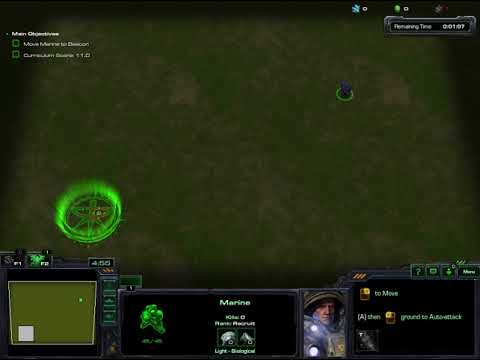
\includegraphics[width=0.75\textwidth]{pysc2_SS}
    \caption{Screenshot of the minigame \emph{MoveToBeacon} in \emph{StarCraft II}.}
    \label{fig:pysc2_SS}
\end{figure}

An \emph{observation} received by the agent in this minigame is given by a $32 \times 32$ grid, representing the entire state of the game, \todo{Is this correct? Or are there actually perhaps only 3 features or something?} giving a total of \emph{$1024$ features}. Each cell in the grid represents a tile in the game. It can have one of three values: a 0 denoting an empty tile, a 1 denoting the army unit controlled by the agent, or a 5 denoting the beacon. The beacon comprises more than one tile, namely a total of $21$ tiles; it comprises five adjecent rows, where the first comprises three adjecent columns, followed by three rows of five columns, followed by a row of three columns. Because of this, the beacon has $27 \cdot 27$ places where it could be, with the army unit having $1003$ tiles left to be. This gives \todo{Is this a correct usage of state-space?} a total state-space of $32 \times 32$ with a cardinality of $27 \cdot 27 \cdot 1003 = 731.187$. An example of such a state observation can be seen in figure \ref{fig:state_example}.

\begin{figure}[h]
    \centering
    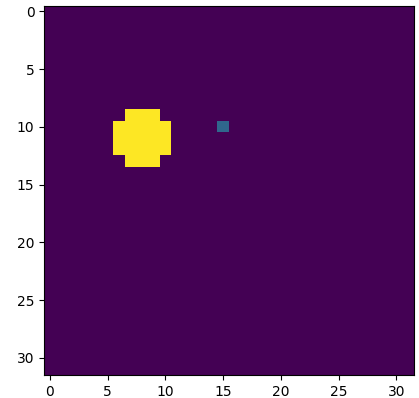
\includegraphics[width=0.75\textwidth]{AE_State_original}
    \caption{A state observation received by the RL agent, for the StarCraft II minigame MoveToBeacon. The yellow cells represent one beacon; the blue cell represents the army unit controlled by the player; all other cells are empty.}
    \label{fig:state_example}
\end{figure}

An \emph{action} taken by the agent is given by an $(x,y)$ coordinate with $x,y \in \{0 .. 31\}$. This denotes the (indices of the) cell in the grid that the army unit will move to.

Lastly, an \emph{episode} takes $120$ seconds. The goal is to move the army unit to the beacon as often as possible in this time limit, each time adding $1$ point to the episode score. At the start of each episode, the beacon and army unit are placed randomly. Whenever the army unit reaches the beacon, only the beacon will be relocated randomly. An agent following a random policy gets a score of about $0-3$ points per episode (again, one point for each time the army unit reaches the beacon), whereas a scripted agent scores about $26-30$ points per episode.

\subsection{Experiments}\label{research-exp}
To examine the effect of the different dimensionality reduction methods, we implemented multiple RL agents using different reduction methods and compared their performance. In this section we will discuss the agents that we used. We will give a general overview here, referring to appendix \ref{appendix} section \ref{appendix-agents} for details on the neural network architectures and hyperparameter settings. 

The first agent mentioned is the vanilla agent, which does not use a dimensionality reduction method, therefore using the full $32 \times 32$ dimensions of the observation. All other agents reduce the dimensionality to $16 \times 16$. This means that the number of features in an observation are reduced from \todo{Again, is this correct?}$1024$ to $256$.

Furthermore, to allow for a fair comparison of their performance, all agents must share as many architectural design choices and hyperparameter settings as possible. This is done by extending the vanilla agent in all other agents. However, one important change must be made. The vanilla agent's neural network receives a $32 \times 32$ input, whereas the other agents receive a $16 \times 16$ input. In all cases, the output dimensions must be $32 \times 32$. This is because the network approximates the Q-function: a valuation of all actions for a given state. Since an action in our environment is defined by the coordinates the army unit must walk to, there are $32 \times 32$ possible actions. To deal with this difference in input dimensions, the first layer of the networks of the non-vanilla agents are modified to increase the dimensionality.\newline

\noindent \textbf{Vanilla agent}\newline
\noindent The vanilla agent is a standard RL agent that does not use any dimensionality reduction. This is the agent that is extended by all other agents. It uses a DDQN strategy, as explained in section \ref{pl-dqn}. %TODO DQN of DDQN?
First, the agent receives an observation from the environment. This observation is passed to its neural network approximating the Q-function. This returns a valuation for each action taken in this state. Then, the agent either chooses the action with the best valuation (i.e. acting greedily) or chooses a random action. An action corresponds to choosing coordinates for the army unit to walk to. Then, the chosen action is performed and we repeat this cycle until the end of the episode, whilst often training the neural network on stored transitions.

The neural network consists of three convolutional layers: the first layer being a Conv2DTranspose, the other two being Conv2D layers. The use of the Conv2DTranpose layer allows for the possibility of changing the dimensionality of the given input. For our vanilla agent, the input dimensions, $32 \times 32$, must remain the same, which is achieved by setting the stride of the first layer to $1$. This way, both the dimensions of the input and the output of the network are $32 \times 32$ (where its input represents the current state observation and its output the action valuation).\newline

\noindent \textbf{PCA agent}\newline
\noindent The PCA agent uses PCA to reduce the dimensionality of the state observations. As mentioned, this is done by extending the vanilla agent: after receiving an observation from the environment, the observation is processed by a PCA component lowering the observation dimensionality from $32 \times 32$ to $16 \times 16$. This latent representation is then used by the agent as if it is the actual observations. This means that it is passed to the network to give an action valuation, as well as being stored in transitions used to train the network.

The output of the network representing the Q-function must remain $32 \times 32$, since we have $32 \cdot 32$ possible actions: one action per coordinate. Therefore, the first layer in the policy network, the aforementioned Conv2DTranspose layer, has a stride of $2$. This changes the dimensions from $16 \times 16$ to $32 \times 32$. 

The PCA component is trained separately before being used by the agent. This is done by training the PCA on $240.000$ previously stored observations. It is important that these observations give a good representation of the environment to get a well trained PCA component. The first $256$ principal components in our PCA (representing a $16 \times 16$ dimensional observation), contain roughly $96\%$ of the information of the original data.\newline

\noindent \textbf{Pre-trained autoencoder agent}\newline
\noindent This agent is very similar to the PCA agent, except instead of using a PCA component, we are using an autoencoder to reduce dimensionality. Just like the PCA component, the autoencoder is pre-trained on the same $240.000$ observations. After this it is used by the agent to reduce the dimensionality of the observation. 

The encoder and decoder of the autoencoder are convolutional neural networks. The encoder uses two Conv2D layers: the first has a stride of $2$, which reduces the dimension to $16 \times 16$. The decoder, which tries to reconstruct the original data, uses three convolutional layers. The first layer is a Cond2DTranspose layer with a stride of $2$, to bring the dimensions back to $32 \times 32$. The other two layers are Conv2D layers. 

The autoencoder is trained by passing batches of observations to the encoder, which performs the dimensionality reduction. Its output is then passed to the decoder which tries to reconstruct the original data. The loss is then calculated by how similar the decoder output is, compared to the original data.

When being used by an agent to reduce the dimensionality of an observation, only the encoder part of the autoencoder is used. The autoencoder is not being trained further while in use by an agent. \newline
 
\noindent \textbf{\todo{I guess "online" is not strictly correct}Online trained autoencoder agent}\newline
\noindent  This agent has the exact same design as the pre-trained autoencoder agent. The only difference is the moment of training the autoencoder. In the pre-trained autoencoder agent, the autoencoder is trained before being used by an agent, using previously stored observations. In this online trained autoencoder agent, we are using an autoencoder that has not been pre-trained; it is being trained while being used by the agent. 

In this case, the agent itself still only uses the encoder part of the autoencoder. However, we now also store observations and pass these to the training method of the autoencoder. This training method is the same as before: passing the observations to the encoder, whose output is passed to the decoder, whose output is compared to the original observation to calculate the loss and train the network.

\noindent \textbf{DeepMDP agent}\newline
\noindent Just like the online trained autoencoder agent, the DeepMDP agent is completely trained while being used by the agent. It also uses an encoder, which has the design as the encoders of the autoencoders: one Conv2D layer with stride $2$ to reduce dimensions and a second Conv2D layer. Differently from the autoencoder though, this encoder is actually part of the agent's network; whereas the autoencoder is a separate network, the DeepMDP simply extends the network of the agent. The agent's network therefore consists of an encoder part and a policy part. This means that when the agent receives an observation from the environment and passes it to its network, it first goes through the encoder whose output is passed to the policy part. In effect this means that the encoder and policy network are now trained on the same loss, using a single optimizer.

Additionally, the DeepMDP makes use of an auxiliary objective to calculate the loss: the transition loss. This transition loss represents the cost of all possible transitions from a given latent representation. This means that its output has dimensions $(32 \times 32) \times 16 \times 16$. The tuple $(32, 32)$ represents the actions that can be taken in the current state, while the other two dimensions, $16 \times 16$ represent the next (predicted) latent observation. It has only one layer, a Conv2D layer, with $32 \times 32$ output channels to represent the action dimensions. Again this network is a part of the agent's network. Consequently, the agent's network consists of three parts: an encoder part, a policy part, and a transition loss part, all trained on the same loss using a single optimizer.

Lastly, a gradient penalty is calculated on all three parts of the network separately. This is represents a Lipschitz-constrained Wasserstein Generative Adversarial Network (lol). Its penalty is used in calculating the loss while training the network. 


\section{Results}\label{research-results}
sectie opzet
\subsection{Research results}
Resultaten van de verschillende agents

\subsection{Discussion}
Resultaten van AE analyse; voordeel pretained benoemen (nml dat je vershcillende agents kan trainen op lagere dimensionality op basis van dezelfde encoder)

